\chapter{Kiirunavaara}

The Kiirunavaara mine located in Kiruna, Sweden and operated by LKAB has struggled with rockbursts since 2008 \autocite[5]{Krekula17}. It is a large underground iron ore mine, with an annual production of 27,5 Mio t crude iron ore in 2018. \autocite[28]{LKABfinance} 
The orebody consists mostly of magnetite.
In \autoref{fig:geo} a map of the geology of the area is given.
%As displayed in \autoref{fig:geo} the ore at Kiirunavaara is mostly magnetite.
It is mined using sub level caving. The current production depth is at around 1100 m.%, the ore body is estimated to continue to depths of 2000 m. %With increasing depth the tensions inside the the rock mass increase as well and the ground becomes more burstprone. Therefore the support systems needs constant updating and development.

%The next step LKAB wants to take is optimizing its surface support concept. The chosen method are drop tests. Drop testing works utilizing gravity to either directly or indirectly transfer kinetic energy to isolated surface support elements. \autocite[1]{Potvin10} Which means that drop weights are dropped from fixed heights onto surface support elements and the mode of failure of these elements together with their maximum capacities among other measured values are studied to gleam insights to help to iterate towards an compromise between rigidity and derformability.
%Drop tests are easily replicable, the largest amount of work is building and handling the test panels. Therefore they are a cheap way to test various set ups. But drop tests have their draw backs. It is only possible to test reinforcement elements, therefore the interaction between surface support and reinforcement support and rock face can not be investigated. The surface support activates the reinforcement support through their connection, insufficient activation of the reinforcement means unused potential, unnecessary cost and premature failure. Overall they are a practical way to optimize surface support under dynamic loading conditions.

\begin{figure}
\centering
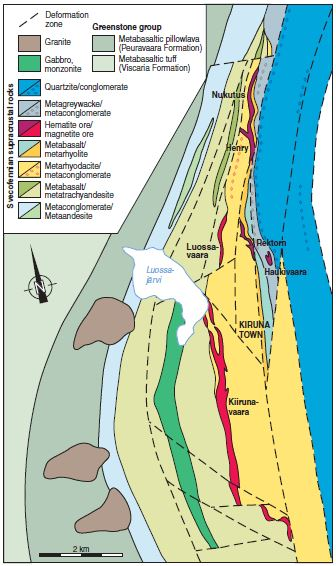
\includegraphics[height = 0.5\textheight]{pics/geo.jpg}
\caption{Geology of the Kirunavaara area \autocite{KirunaGeo}}
\label{fig:geo}
\end{figure}

\section{Transition from Seismically Inactive to Seismically Active}

Up until 2007 only minor rockbursts happened at Kiirunavaara mine which were also confined to a small area within the mine. After 4 large seismic events and corresponding rockbursts on 2 to 3 levels between late 2007 and early 2008 it became obvious that rockbursts were no longer exceptions. %To understand the problem a network of geophones was built, as displayed in \autoref{fig:phone} the amount of geophones increased substantially. \autocite{dahner12}

\begin{comment}
\begin{figure}
    \centering
    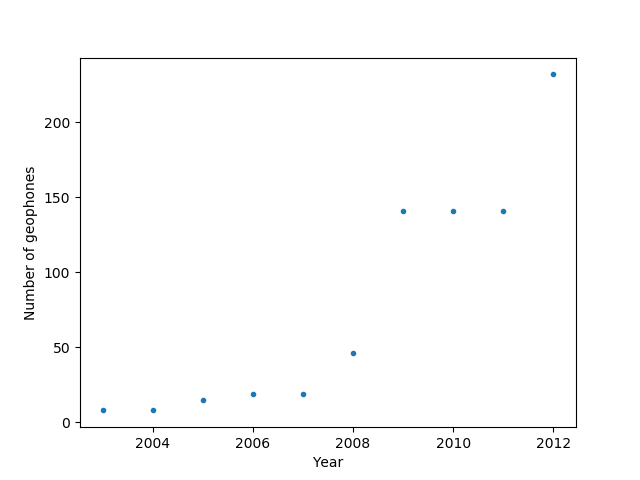
\includegraphics{pics/geophones.png}
    \caption{Increase in number of active geophones between 2004 and 2012 after \autocite[4]{dahner12}}
    \label{fig:phone}
\end{figure}
\end{comment}

Measures to decrease the vulnerability to rock bursts were taken. For example the production sequence was optimised and procedures to close vulnerable areas of the mine were implemented.
The rock support system used so far only had to provide static support, it consisted mostly of 3 - 4 cm of shotcrete and grouted rebar. \autocite[9]{dahner12}

\section{Current Support System}

\begin{figure}
    \centering
    \begin{tikzpicture}
%current support system

%membrane
\draw (0,0) arc [radius = 8cm, start angle= 120, end angle= 60];
\draw (0,-1) arc [radius = 8cm, start angle= 120, end angle= 60];
\draw [thick,dash pattern={on 7pt off 2pt on 1pt off 3pt}] (0,-1.3) arc [radius = 8cm, start angle= 120, end angle= 60];
\path (0,-1.8) arc [radius = 8cm, start angle= 120, end angle= 60] 
coordinate [pos = 0.2] (left)
coordinate [pos = 0.35] (leftmid)
coordinate [pos = 0.5] (mid)
coordinate [pos = 0.65] (rightmid)
coordinate [pos = 0.8] (right);

%bolts
\draw 
(left) -- ++ (110:4)
(leftmid) -- ++ (100:10)
(mid) -- ++ (90:4)
(rightmid) -- ++ (80:10)
(right) -- ++ (70:4);

%text
\node[right] at (8.5,0.5) {rock};

\node[right] at (8.5,-0.5) {FRS};

\node[right] at (8.5,-1.3) {welded mesh};

\node at (4,-1.8) {excavation};

\node at (4,7) {cable bolts};

\node at (7,3) [right] {dynamic bolts};
\end{tikzpicture}
    \caption{Cross section of the current support system}
    \label{fig:cross}
\end{figure}

\begin{figure}
    \centering
    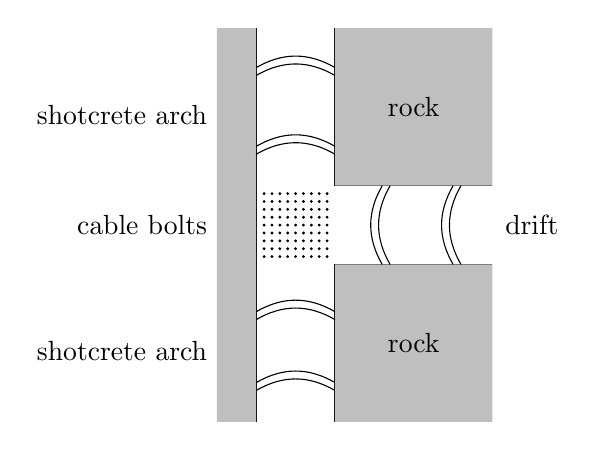
\begin{tikzpicture}

%drift
\draw (0,0) -- (0,2) -- (2,2);
%\draw (-1,0) -- (-1,2) -- (-3,2);
\draw (2,3) -- (0,3) -- (0,5);
%\draw (-3,3) -- (-1,3) -- (-1,5);
\draw (-1,0) -- (-1,5);

%rock
\path [fill = lightgray]
(0,0) -| (2,2) -| cycle
(2,3) -| (0,5) -| cycle
(-1.5,0) -| (-1,5) -| cycle; 

%cable bolts
\foreach \x in {0.1,0.2,...,0.9}{
\foreach \y in {0.1,0.2,...,0.9}{
\draw[fill = black] 
(-1+\y,2+\x) circle [radius=0.01]
;}}

%shotcrete arch
\draw (0,0.5) to [bend right](-1,0.5)
(0,0.4) to [bend right](-1,0.4);
\draw (0,1.3) to [bend right](-1,1.3)
(0,1.4) to [bend right](-1,1.4);

\draw (0,4.5) to [bend right](-1,4.5)
(0,4.4) to [bend right](-1,4.4);
\draw (0,3.5) to [bend right](-1,3.5)
(0,3.4) to [bend right](-1,3.4);

\draw (1.5,2) to [bend left](1.5,3)
(1.6,2) to [bend left](1.6,3);
\draw (0.7,2) to [bend left](0.7,3)
(0.6,2) to [bend left](0.6,3);

%text
\node at (1,1) {rock};
\node at (1,4) {rock};
\node at (2.5,2.5) {drift};
\node [left] at (-1.5,2.5) {cable bolts};
\node [left] at (-1.5,0.9) {shotcrete arch};
\node [left] at (-1.5,3.9) {shotcrete arch};

%\node [right] at (0,3.5) {cable bolts};
%\node [right] at (0,1) {shotcrete arch};
%\node [right] at (-3,2.5) {drift};
\end{tikzpicture}
    \caption{Top view of the placement of shotcrete arches and cable bolts}
    \label{fig:arch}
\end{figure}

The support system developed in response to Kiirunavaara mine becoming seismically active has evolved and solidified into the support system currently in use. It consists mainly of 10 cm of fibre reinforced shotcrete, with welded mesh on top with a wire diameter of \o 5,5 mm and and an aperture of 75 mm and 3 m long dynamic bolts with 1 m spacing and > 7 m long cable bolts in the roof of 3 - way and 4 - way intersections or where the geology requires it. See \autoref{fig:cross}.  Especially burst prone areas are supported with concrete arches with a thickness of 200 mm. The bolts are square spaced and mesh is connected with 3 squares of overlap. % as displayed in \autoref{fig:mesh}.
Pillars between ore passes are reinforced with steel straps called "Fjällband" if the operational rock mechanic engineers recommend it. \autocite{Jonson15}
%%%% maybe fix that sentence?

\section{Requirements of Support System}
This support system and any change made to it have to fulfill several requirements.

\subsection{Lifetime}

The most important one is longevity. A support system has to be serviceable for as long as the excavation is expected to be open. See \autoref{tab:life}. Please note that active production area refers to drifts with ongoing production and that support used in the primary infrastructure must always undergo long-term tests. After the times mentioned the support system has to retain 85 \% of the initial strength requirements. \autocite[3]{Winsa18}

\begin{table}
    \centering
    \begin{tabular}{ll}
    \toprule
        Type of use & Lifetime in years \\
    \midrule
         Production area & 10  \\
         Active production area & 2 \\
         Main haulage level & 20 \\
    \bottomrule
    \end{tabular}
    \caption{Approximate lifetime expectation at Kiirunavaara Mine after \textcite[3]{Winsa18}}
    \label{tab:life}
\end{table}

\subsection{Surface Support}

%The strength requirements for surface support are entirely based on quasi-static tests. 
The quasi static strength of FRS is tested and evaluated using \autocite{c1550}. 
For mesh only welded mesh has a regulated testing procedure.
The dynamic capabilities are assumed based on \textcite{Potvin10}.
Blast tests conducted by \autocite[9]{shirzadegan16} give an energy absorption capacity of 4 \(\frac{\text{kJ}}{\text{m}^2}\) for this combination.
%The energy absorption of FRS and mesh are assumed to be 7,5 and 2,5 \(\frac{\text{kJ}}{\text{m}^2}\). After a simple addition that means that the current support system supposedly has energy absorption capabilities of 10 \(\frac{\text{kJ}}{\text{m}^2}\). \autocite[4]{Biruk13}

\subsection{Reinforcement Support}

For bolts a mix of static and dynamic tests are required. These are conducted by CanmetMINING. \autocite{Winsa18}